\section{Ziel}
\label{sec:Ziel}

Ziel dieses Versuchs ist die Bestimmung der Wellenlänge eines Lasers mit Hilfe eines Michelson-Interferometers. 
Zudem soll der Brechungsindex von Luft ermittelt werden. 

\section{Theorie}
\label{sec:Theorie}

In diesem Kapitel wird zunächst auf die Natur des Lichts und seine Interpretation als Welle in diesem Versuch eingegangen.
Auf dieser Grundlage werden die Phänomene erläutert, die am Michelson-Interferometer untersucht werden können. 
Zudem wird der Aufbau und die Verwendung des Michelson-Interferometers erklärt. 
\subsection{Wellencharakter des Lichts und Interferenz}
\label{ssec:Interferenz}

Verschiedene Versuche zur Natur des Lichts liefern Ergebnisse, die je nach Versuchsanordnung eine Beschreibung des 
Lichts als Welle oder Teilchen (Korpuskel) erfordern. Die gemeinsame Erklärung dieser klassisch unvereinbaren Ergebnisse 
wird durch die Quantenelektrodynamik ermöglicht. Es werden dabei Korpuskel- und Wellenmodell als Grenzfälle
der Quantenelektrodynamik verstanden. Betrachtet man wie in diesem Versuch die Ausbreitung von Licht im Vakuum, stellt das 
Wellenmodell die geeignete Näherung dar, um die auftretenden Phänomene zu beschreiben und zu erklären, insbesondere 
das Phänomen der Interferenz. 

Nimmt man also an, dass Licht eine elektromagnetische Welle ist und betrachtet den einfachsten Fall einer ebenen Welle, 
kann die Ort- und Zeitabhängigkeit der elektrischen Feldstärke $\vec{E}$ in der Form
\begin{equation}
    \vec{E}(x,t) = \vec{E_0} \cos\left(kx - \omega t - \delta\right)
\label{eqn:wave}
\end{equation}
beschrieben werden. Hier steht $k = \frac{2\pi}{\lambda}$ für die Wellenzahl, $\omega$ für die Kreisfrequenz und 
$\delta$ für einen Phasenwinkel in Bezug auf Orts- und Zeitnullpunkt. Es gilt das Prinzip der linearen Superposition.
Werden in einem Punkt im Raum $n$ Lichtwellen überlagert, ist die Gesamtfeldstärke des resultierenden elektrischen Feldes 
in diesem Punkt die Summe der Feldstärken der $n$ Lichtwellen, die überlagert werden. Es gilt also 
$E_\text{ges} = E_1 + E_2 + ... + E_\text{n}$. Diese Änderung der Gesamtamplitude bei der Überlagerung mehrerer Wellen nach dem 
Superpositionsprinzip wird als Interferenz bezeichnet. 

Aufgrund der hohen Lichtfrequenz in der Größenordnung $\SI{e15}{\hertz}$ ist die elektrische Feldstärke in der Praxis
nicht direkt messbar, weshalb stattdessen die Intensität gemessen wird. Aus den Maxwell-Gleichungen kann hergeleitet 
werden, dass Intensität und Energie einer elektromagnetischen Welle über die Beziehung 
\begin{equation}
    I = \text{const} \cdot |\vec{E}|^2
\end{equation}
miteinander verknüpft sind. Für die Summe der Intensitäten zweier elektromagnetischer Wellen in einem Punkt im Raum
gilt demnach
\begin{equation}
    I_\text{ges} = 2 \text{const} \vec{E_0}^2 \cos\left(1 + \delta_2 - \delta_1\right) .
\end{equation}
Die Gesamtintensität zweier Wellen, die in einem Raumpunkt überlagert werden, ist also nicht einfach die Summe der Einzelintensitäten der 
überlagerten Wellen $2 \text{const} \vec{E_0}^2$, sondern hängt auch vom Phasenunterschied der Wellen ab. 
Der Interferenzterm
\begin{equation}
    2 \text{const} \vec{E_0}^2 \cos\left(\delta_2 - \delta_1\right), 
\end{equation}
beschreibt das Interferenzverhalten der überlagerten Wellen und kann je nach Phasenlage der Wellen zueinander Werte 
zwischen $ -2 \text{const} \vec{E_0}^2$ und $2 \text{const} \vec{E_0}^2$ annehmen. 
Er nimmt den Wert 0 an, wenn $\delta_2 - \delta_1$ ein ungerades Vielfaches von $\pi$ ist. 

\subsection{Bedingungen für Interferenz und der Begriff der Kohärenz}
\label{ssec:kohärenz}

Im Allgemeinen lässt sich keine Interferenz beobachten, wenn Licht aus zwei verschiedenen Lichtquellen überlagert wird.
Grund dafür ist die Natur der Entstehung von Licht. Gehen angeregte Atome in ihren Grundzustand zurück, wird dabei Energie in 
Form von elektromagnetischen Wellen emittiert. Da diese Wellen eine endliche Länge haben und ihre Emission über die Zeit
einer statistischen Verteilung unterliegt, verschwindet der Interferenzterm bei Mittelung über einen hinreichend großen 
Zeitraum. Das von zwei verschiedenen Lichtquellen emittierte Licht ist also nicht interferenzfähig und wird als
inkohärent bezeichnet. 

Kohärentes Licht zeichnet sich hingegen dadurch aus, dass gemäß \autoref{eqn:wave} k, $\omega$ und $\delta$ für alle emittierten Wellenzüge
konstant sind. Die Erzeugung von kohärentem Licht ist mit Hilfe von Lasern möglich. 

Es ist jedoch mit konventionellen Lichtquellen möglich, Interferenzeffekte zu beobachten. Dafür wird Licht aus einer 
Lichtquelle mit Hilfe eines Strahlteilers oder einer Doppelblende in zwei getrennte Strahlenbündel aufgeteilt. Die 
Verwendung eines oder mehrerer Spiegel ermöglicht es, dass die beiden Strahlen nach dem Durchlaufen unterschiedlich 
langer Strecken in einem Punkt $P$ wieder zusammengeführt werden. Die aus dem Wegunterschied resultierende 
Phasendifferenz führt hier zu Interferenz. 
Wird der Wegunterschied der beiden Strahlen allerdings zu groß gewählt, tritt keine Interferenz mehr auf. Dies ist damit
zu begründen, dass der Emissionsvorgang eines Lichtzuges nur eine begrenzte Zeit beansprucht und dementsprechend auch die
Länge des Wellenzuges endlich ist. Ist der Wegunterschied der beiden Strahlen größer als die Länge der Wellenzüge, treffen
die Wellenzüge also zu unterschiedlichen Zeitpunkten im Punkt $P$ auf und es kann keine Interferenz auftreten. Die
Länge, bei der im Punkt $P$ gerade keine Interferenz mehr auftritt, wird als Kohärenzlänge $l$ bezeichnet. 
Die Kohärenzlänge ist definiert als
\begin{equation}
    l = N \lambda ,
\end{equation}
wobei $N$ die Zahl der maximal beobachtbaren Interferenzmaxima im Punkt $P$ ist. 

\subsection{Das Michelson-Interferometer}
\label{ssec:Michelson}

Der Aufbau des Michelson-Interferometers ist in \autoref{fig:michelson} skizziert. 

\begin{figure}[h]
    \centering
    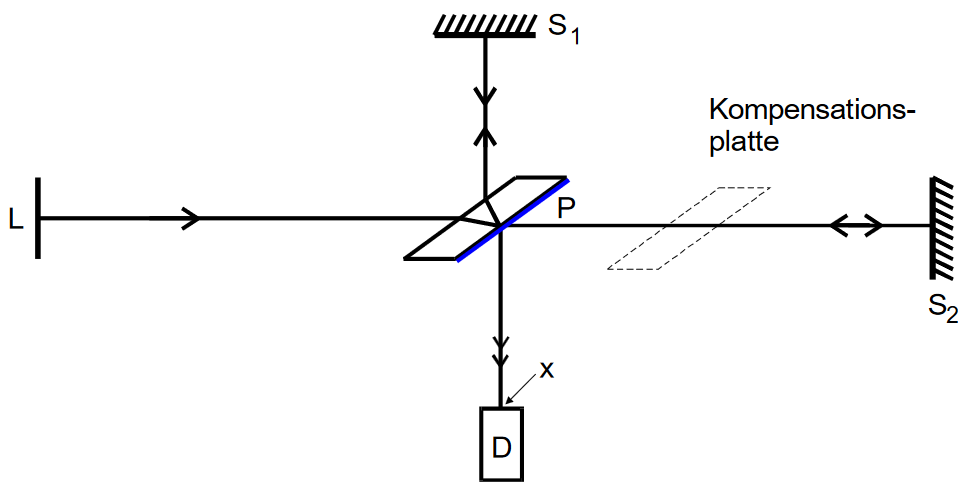
\includegraphics[width=6cm]{content/michelson.png}
    \caption{Schematischer Aufbau des Michelson-Interferometers. \cite{sample}}
    \label{fig:michelson}
  \end{figure}

Die Strahlteilung erfolgt mit Hilfe eines semi-permeablen Spiegels, der in \autoref{fig:michelson} mit $P$ gekennzeichnet
ist. Ein Teil des Lichts wird an diesem Spiegel zu Spiegel $S1$ reflektiert, während der andere Teil das semi-permeable 
Material durchdringt und Spiegel $S2$ erreicht. Beide Strahlen werden am jeweiligen Spiegel reflektiert und erreichen 
erneut den Spiegel $P$, an dem beide Strahlen wiederum geteilt werden. Für die Untersuchung der Interferenzphänomene sind
lediglich die Anteile relevant, die den Spiegel passieren und zum Detektor $D$ gelangen. Entscheidend ist dabei, dass
die beiden Strahlenbündel kohärent sind, ihr optischer Wegunterschied also kleiner als die Kohärenzlänge der Lichtquelle ist.
Dies kann realisiert werden, indem die Strecken $\overline{PS1}$ und $\overline{PS2}$ identisch gewählt werden und zudem eine
Kompensationsplatte zwischen $P$ und $S2$ gebracht wird, die die selbe Dicke wie der semi-permeable Spiegel hat und aus einem
Material gefertigt ist, welches einen identischen Brechungsindex hat. Die Kompensationsplatte wird benötigt, da der Lichtstrahl,
der die Strecke $\overline{PS1}$ zurücklegt, auf seinem Weg von Lichtquelle zu Detektor insgesamt drei mal den semi-permeablen
Spiegel passiert, während der andere Lichtstrahl, der die Strecke $\overline{PS2}$ zurücklegt, auf seine Weg zum Detektor nur einmal
den semi-permeablen Spiegel nur einmal passiert. 

Unter diesen Voraussetzungen stellt sich für $\overline{PS1}$ = $\overline{PS2}$ am Detektor ein Gangunterschied von $\frac{\lambda}{2}$ 
zwischen den Lichtstrahlen ein, was zu destruktiver Interferenz führt. Verschiebt man nun einen Spiegel um die Strecke
d, ändert sich die detektierte Intensität. Es gilt die Gleichung
\begin{equation}
    d = z \frac{\lambda}{2}, 
\end{equation}
wobei z die Zahl der Helligkeitsmaxima ist. 

Eine weitere Möglichkeit zur Erzeugung eines optischen Wegunterschieds ist das Einbringen eines Mediums der Länge $b$ mit einem 
Brechungsindex $n + \Delta n$ in den Weg eines der beiden Lichtstrahlen, exemplarisch dargestellt in \autoref{fig:index}. 

\begin{figure}[h]
    \centering
    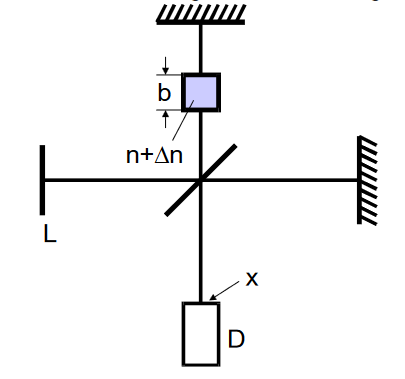
\includegraphics[width=12cm]{content/brechungsindex.png}
    \caption{Aufbau zur Messung kleiner Brechungsindexunterschiede mit dem Michelson-Interferometer. \cite{sample}}
    \label{fig:index}
  \end{figure}

Der optische Wegunterschied der beiden Strahlen beträgt dann $\Delta N b$. 
Nutzt man als solches Medium ein Gasgemisch, welches in einer Zelle in den Strahlengang eingebracht
wird, lässt sich der Weglängenunterschied $\Delta N b$ erhöhen, indem man die Zelle evakuiert oder den Druck $p$ in dieser erhöht.
Wird der optische Weglängenunterschied auf diese Weise stetig erhöht, lassen sich am Detektor $z$ Interferenzmaxima erkennen.
Es gilt das Verhältnis
\begin{equation}
    b \cdot  \Delta n = \frac{z\lambda}{2} .
    \label{eqn:deltan}
\end{equation} 

Aus der klassischen Dispersionstheorie folgt die Formel
\begin{equation}
    n = \sqrt{1 + f(\lambda) \cdot N}
    \label{eqn:dispersion}
\end{equation}
herleiten. Sie beschreibt das Verhältnis zwischen dem Brechungsindex $n$ eines Materials und der Zahl $N$ der erzwungenen 
Schwingungen angeregten Dipole pro Volumeneinheit. Für Licht im sichtbaren Bereich gilt $fN \ll 1$ kann \autoref{eqn:dispersion}
zu 
\begin{equation}
    n = 1 + \frac{f}{2} N
\end{equation}
genähert werden. Für die in diesem Versuch untersuchten Druckbereiche darf weiterhin angenommen werden, dass die verwendeten Gase 
sich wie ideale Gase verhalten. Die Abhängigkeit der Zahl $N$ der vorhandenen Moleküle pro Volumeneinheit in Abhängigkeit von Druck $p$ und 
Temperatur $T$ lässt sich durch
\begin{equation}
    N(p,T) = \frac{p}{T} \frac{T_0}{p_0} N_\text{L}
\end{equation}
beschreiben. Hierbei sind $T_0 = \SI{273,15}{\kelvin}$ und $p_0 = \SI{1013,2}{\bar}$ Normaltemperatur und -druck. 
Die Loschmidtsche Zahl $N_\text{L}$ ist die Zahl der Moleküle, die sich unter diesen Normalbedingungen in 1 Mol eines
Gases enthalten sind. 
Für den Unterschied des Brechungsindex, der sich bei Änderung des Drucks von $p$ zu $p'$ ergibt, gilt demnach
\begin{equation}
    \Delta n(p,p') = \frac{f}{2} N_\text{L} \frac{T_0}{p_0} \frac{1}{T} (p-p') .
\end{equation}
Der Brechungsindex eines Materials unter Normalbedingungen kann mit
\begin{equation}
    n(p_0,T_0) = 1 + \Delta n (p,p') \frac{T}{T_0} \frac{p_0}{p-p'}
\end{equation}
bestimmt werden. Setzt man in diese Gleichung nun noch \autoref{eqn:deltan} ein, folgt für die endgültige Formel zur Bestimmung des
Brechungsindex aus Druckvariation
\begin{equation}
    n(p_0, T_0) = 1 + \frac{z\lambda}{2b} \frac{T}{T_0} \frac{p_0}{p-p'} .
\end{equation}